\section{Kinematic Simulation} 
    This section contains the plots of simulated kinematic parameters (i.e. displacement, velocity and acceleration) for the output component. The independent axis is either Time or Motion of the input link.

    \subsection{Output Component}
        \subsubsection{Simulated and Expected displacement profile}
            \begin{figure}[hbt!]
                \centering
                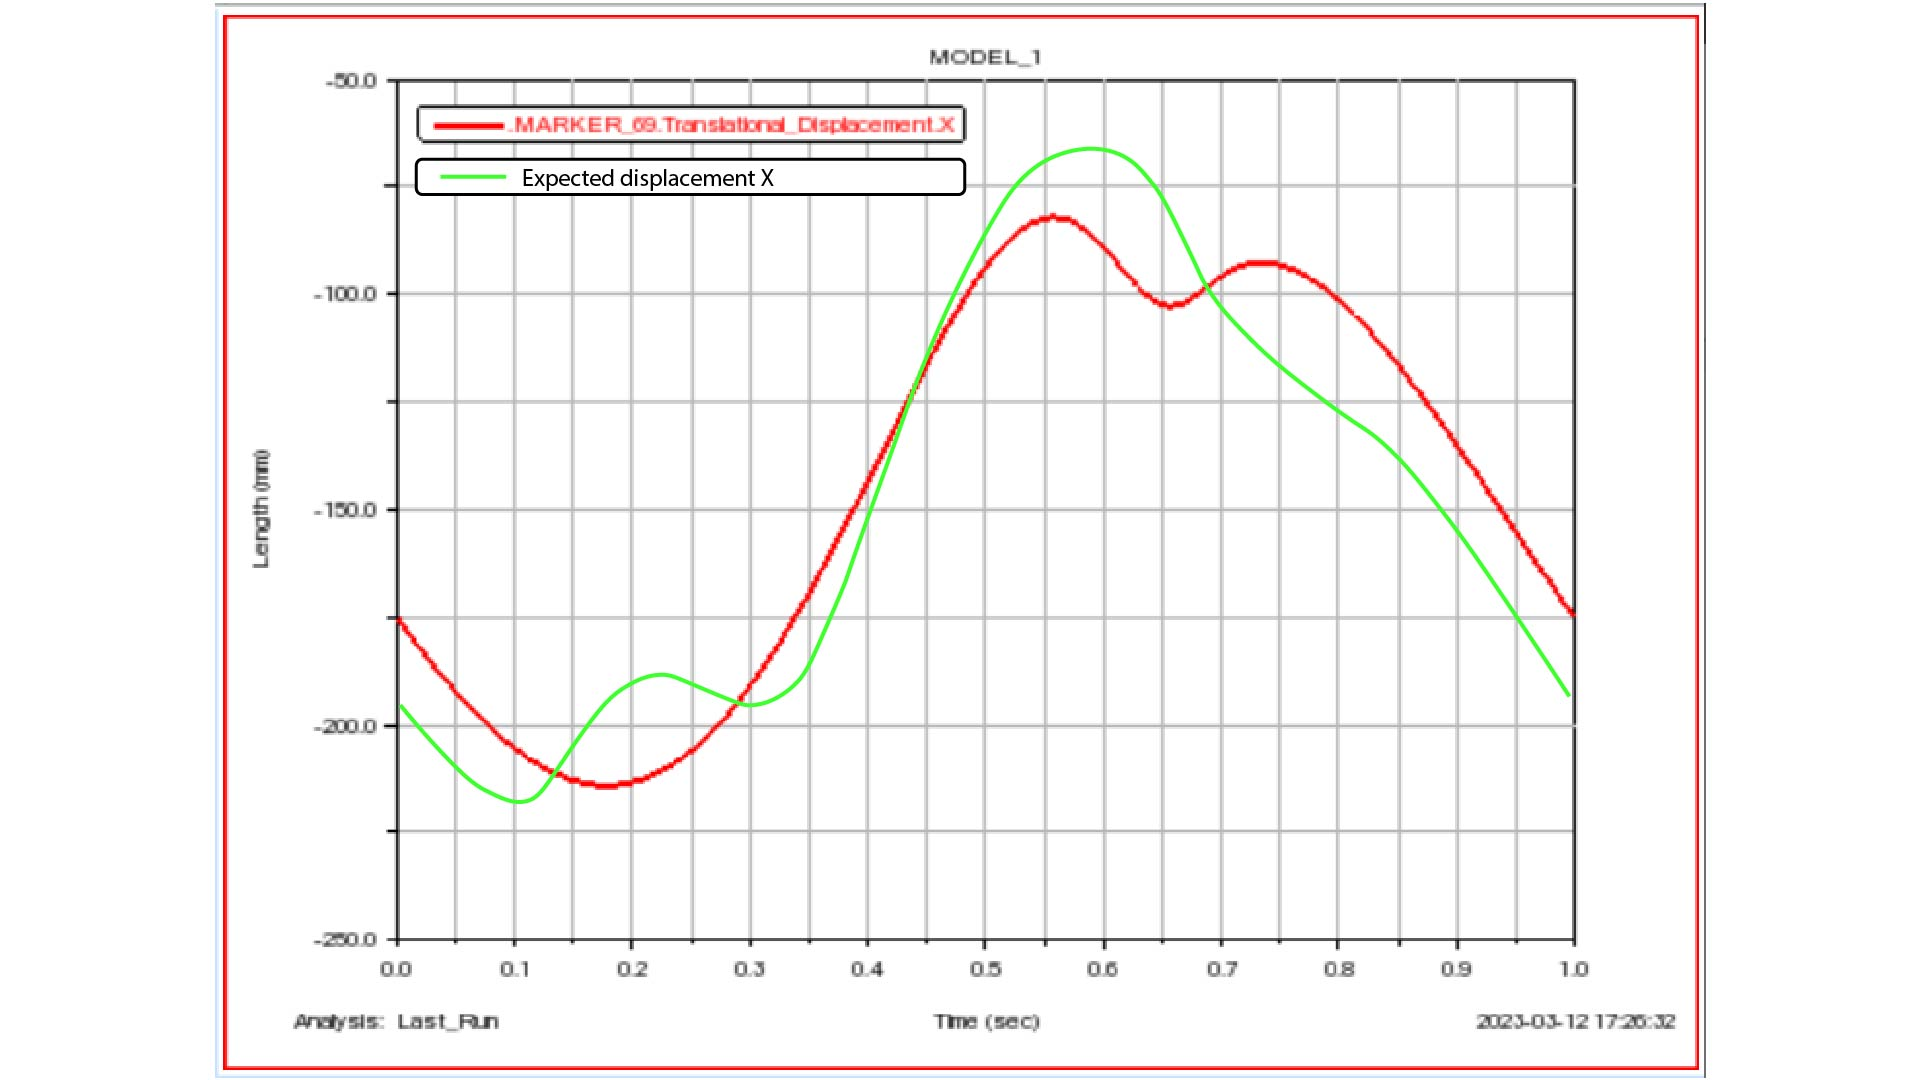
\includegraphics[width=0.9\columnwidth]{Images/x_disp madhav-01.jpg}
                \caption{X displacement vs time}
                \label{fig:x_disp}
            \end{figure}

            \begin{figure}[hbt!]
                \centering
                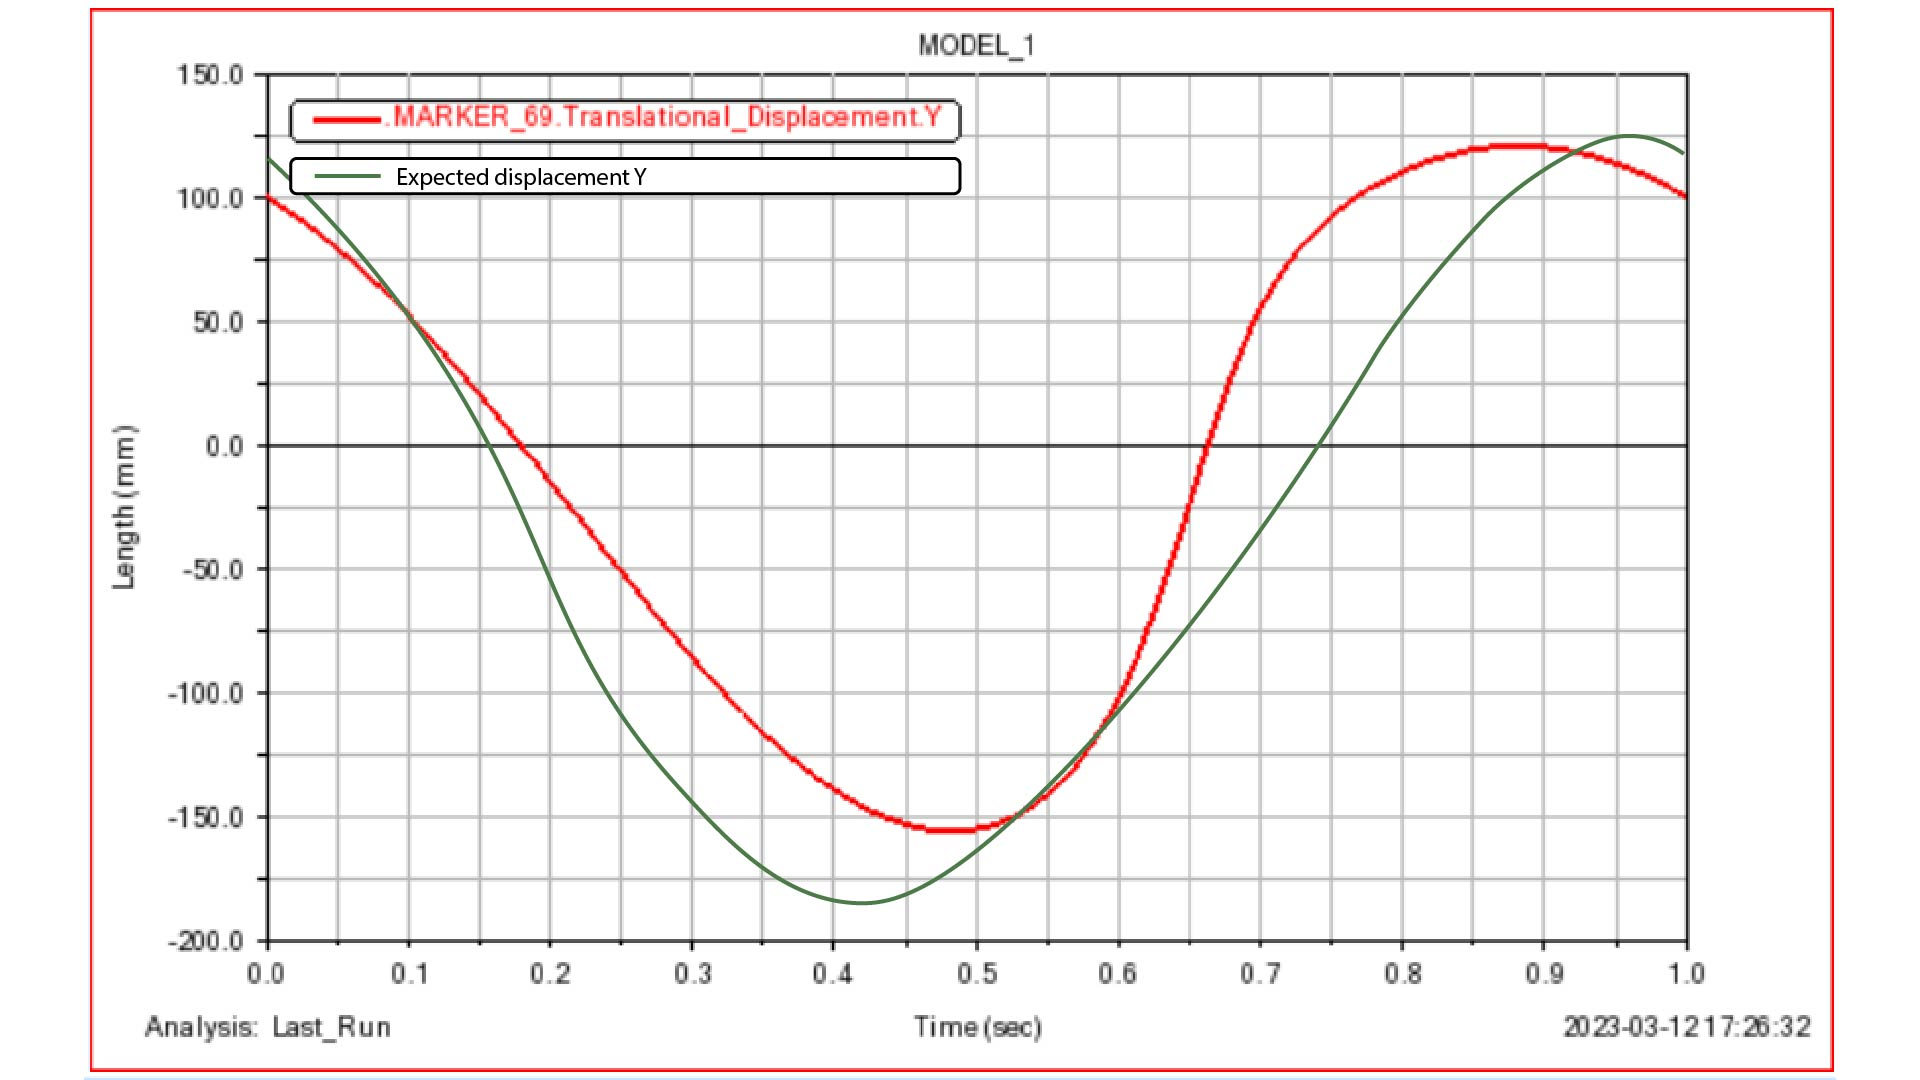
\includegraphics[width=0.9\columnwidth]{Images/height_variation madhav-01.jpg}
                \caption{Height (Y) vs time}
                \label{fig:y_disp}
            \end{figure}

        \subsubsection{Simulated and Expected velocity profile}
            \begin{figure}[hbt!]
                \centering
                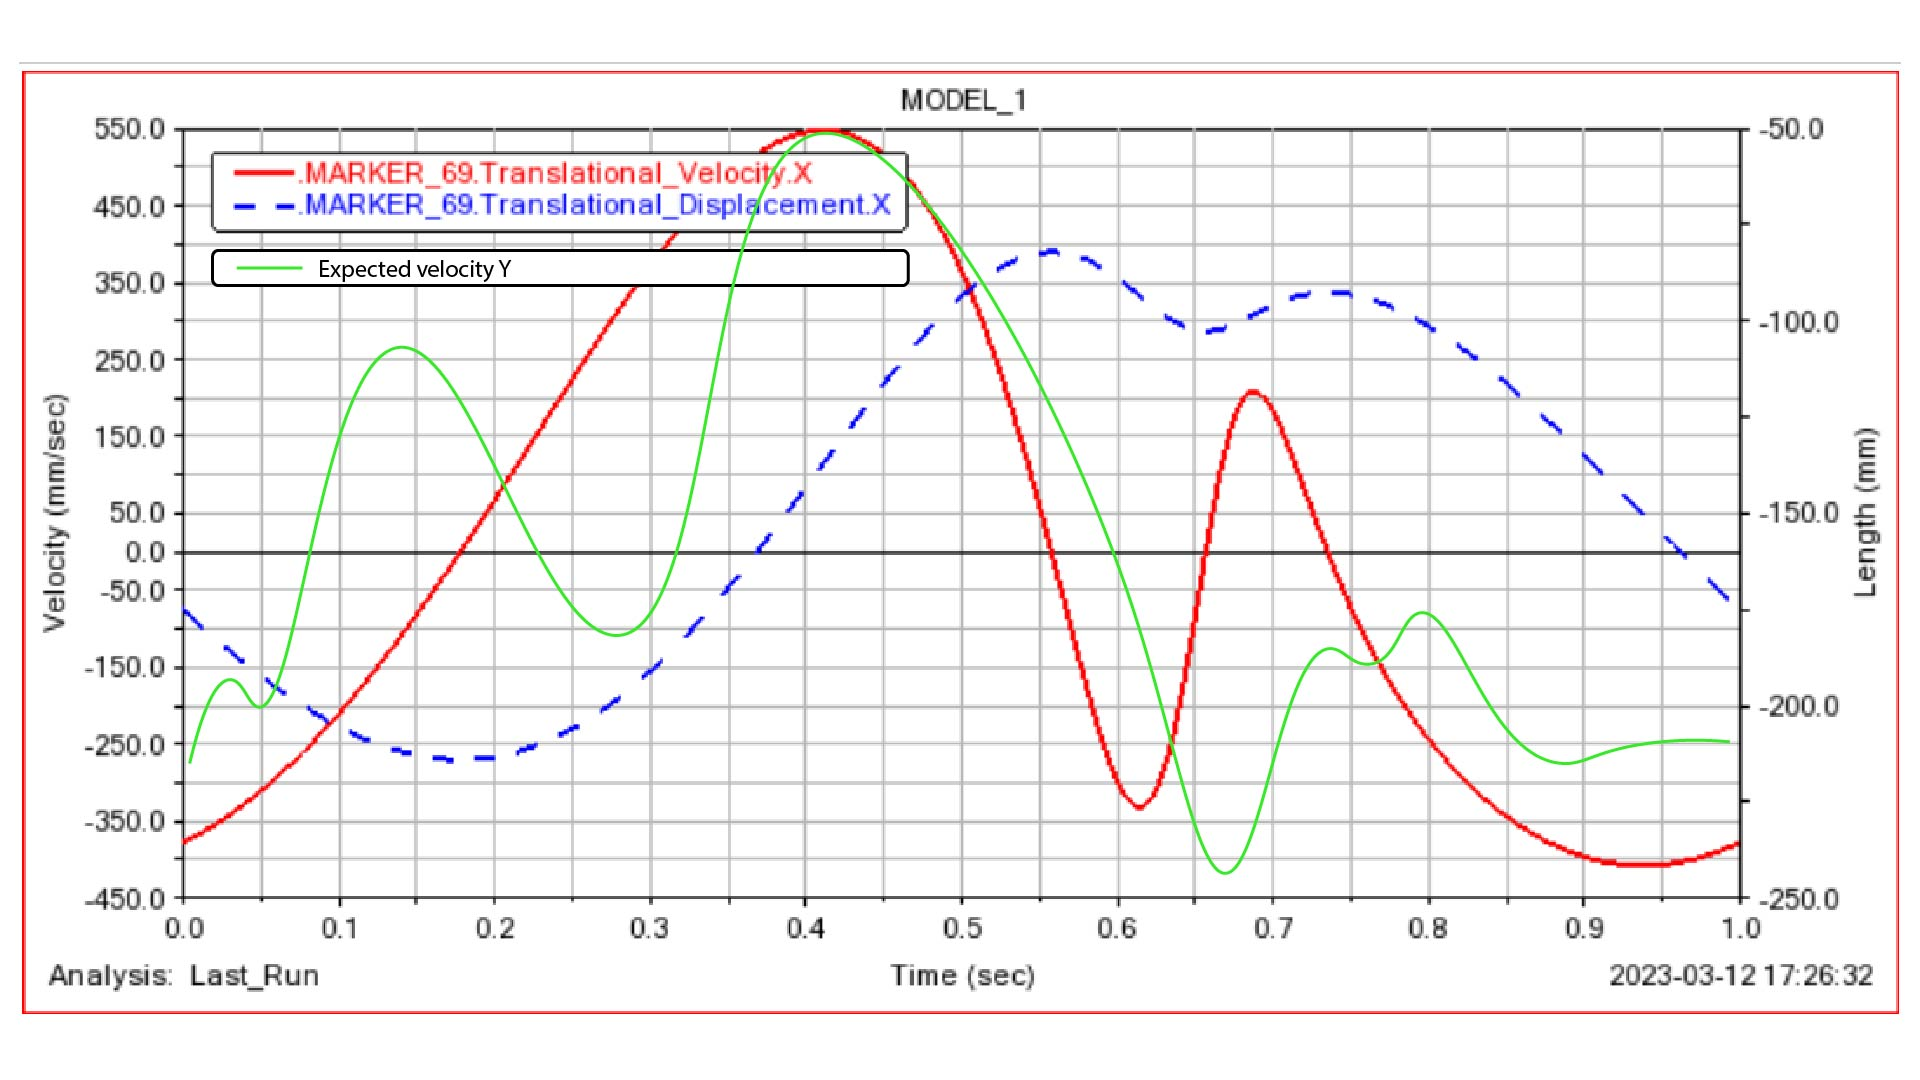
\includegraphics[width=0.9\columnwidth]{Images/x_vel madhav-01.jpg}
                \caption{X Velocity vs time}
                \label{fig:x_vel}
            \end{figure}

            \begin{figure}[hbt!]
                \centering
                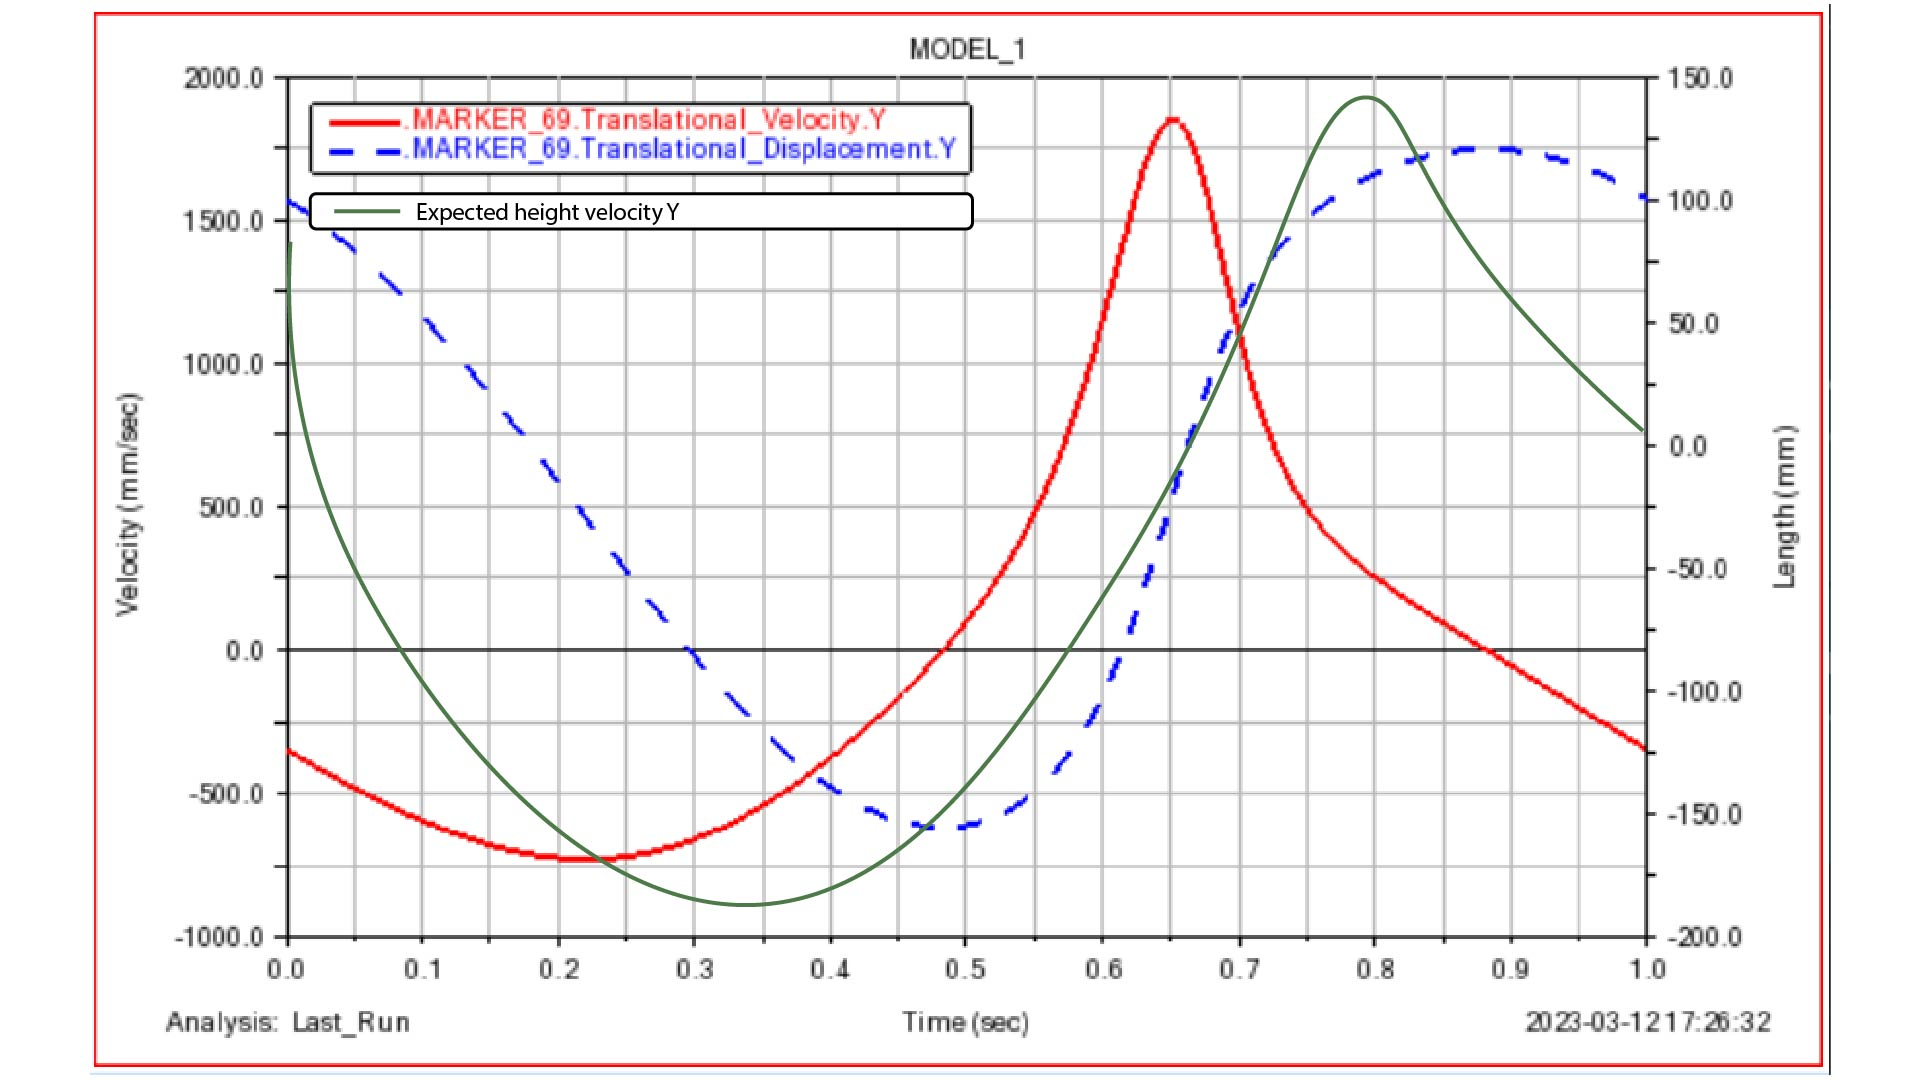
\includegraphics[width=0.9\columnwidth]{Images/height_velocity madhav-01.jpg}
                \caption{Y Velocity vs time}
                \label{fig:y_vel}
            \end{figure}

        \subsubsection{Simulated and Expected acceleration profile}
            \begin{figure}[hbt!]
                \centering
                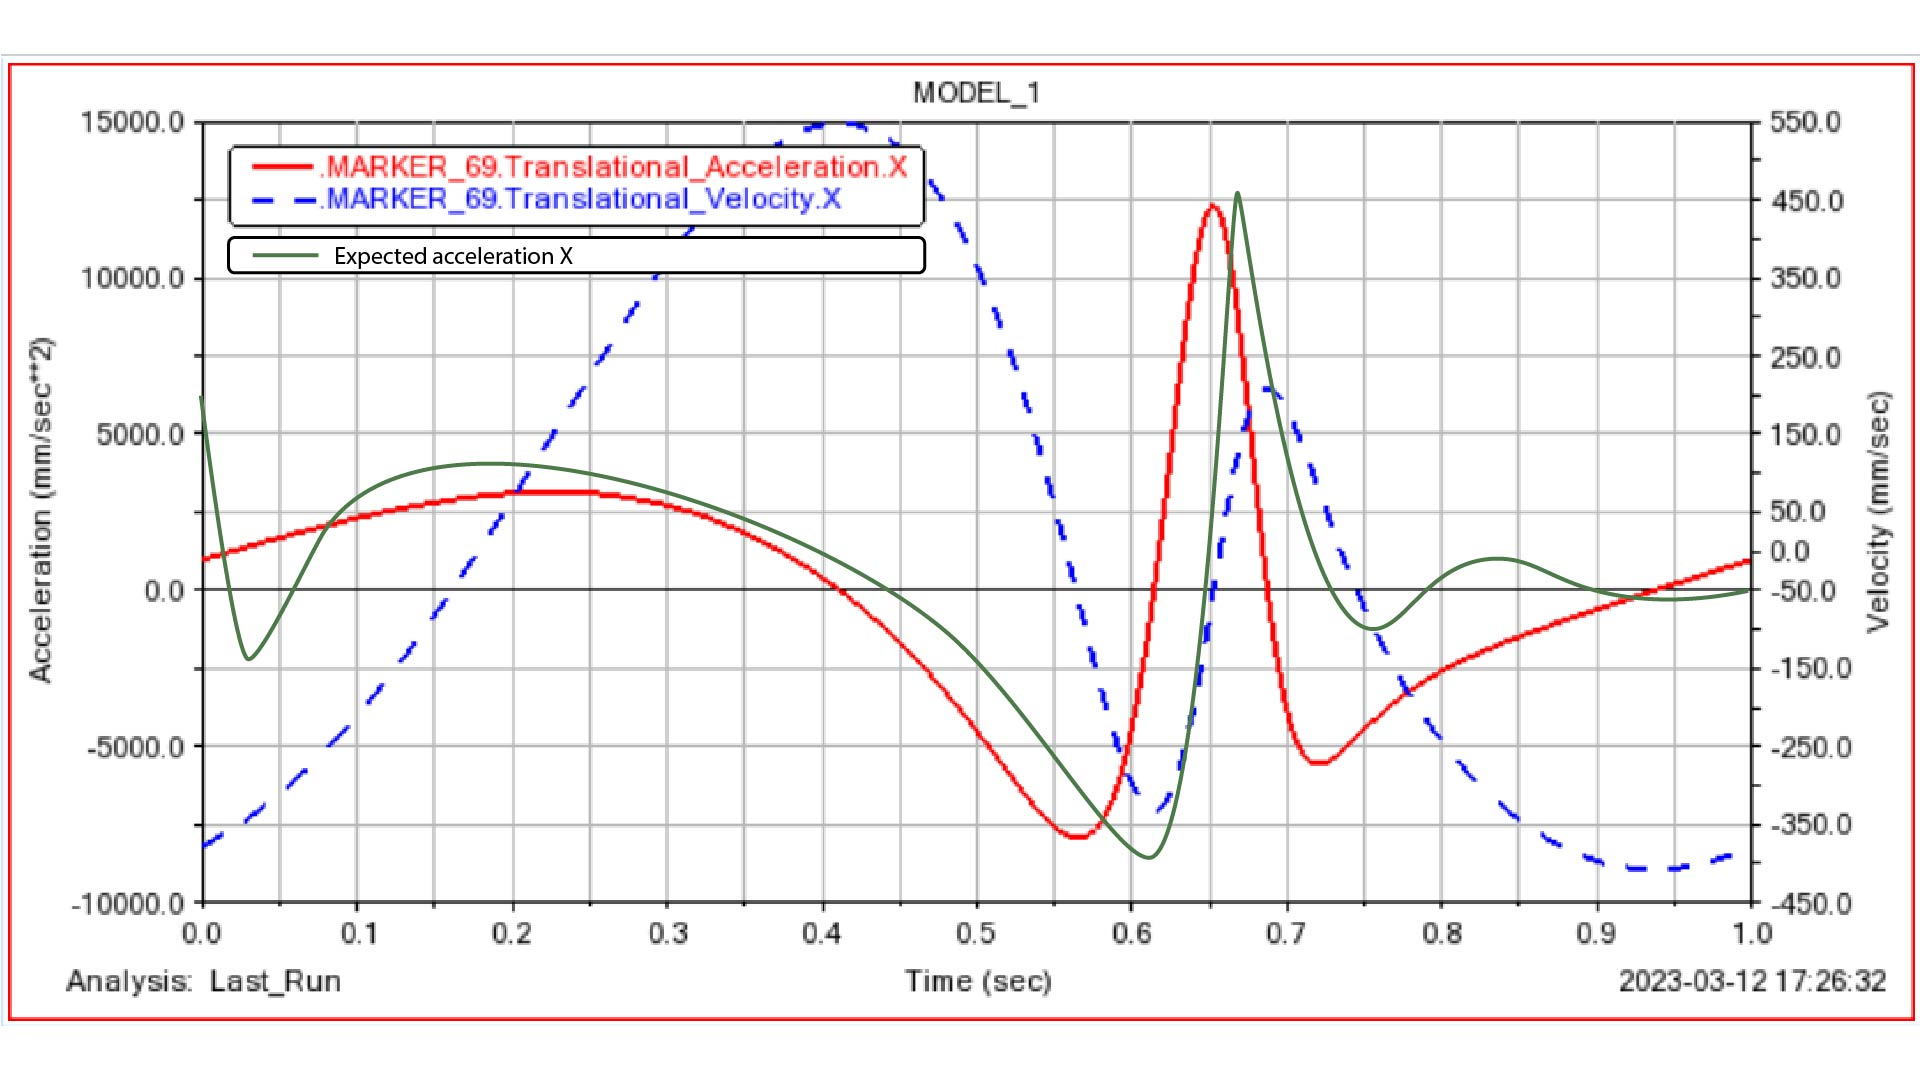
\includegraphics[width=0.9\columnwidth]{Images/x_acc madhav-01.jpg}
                \caption{X Acceleration cs time}
                \label{fig:x_acc}
            \end{figure}

            \begin{figure}[hbt!]
                \centering
                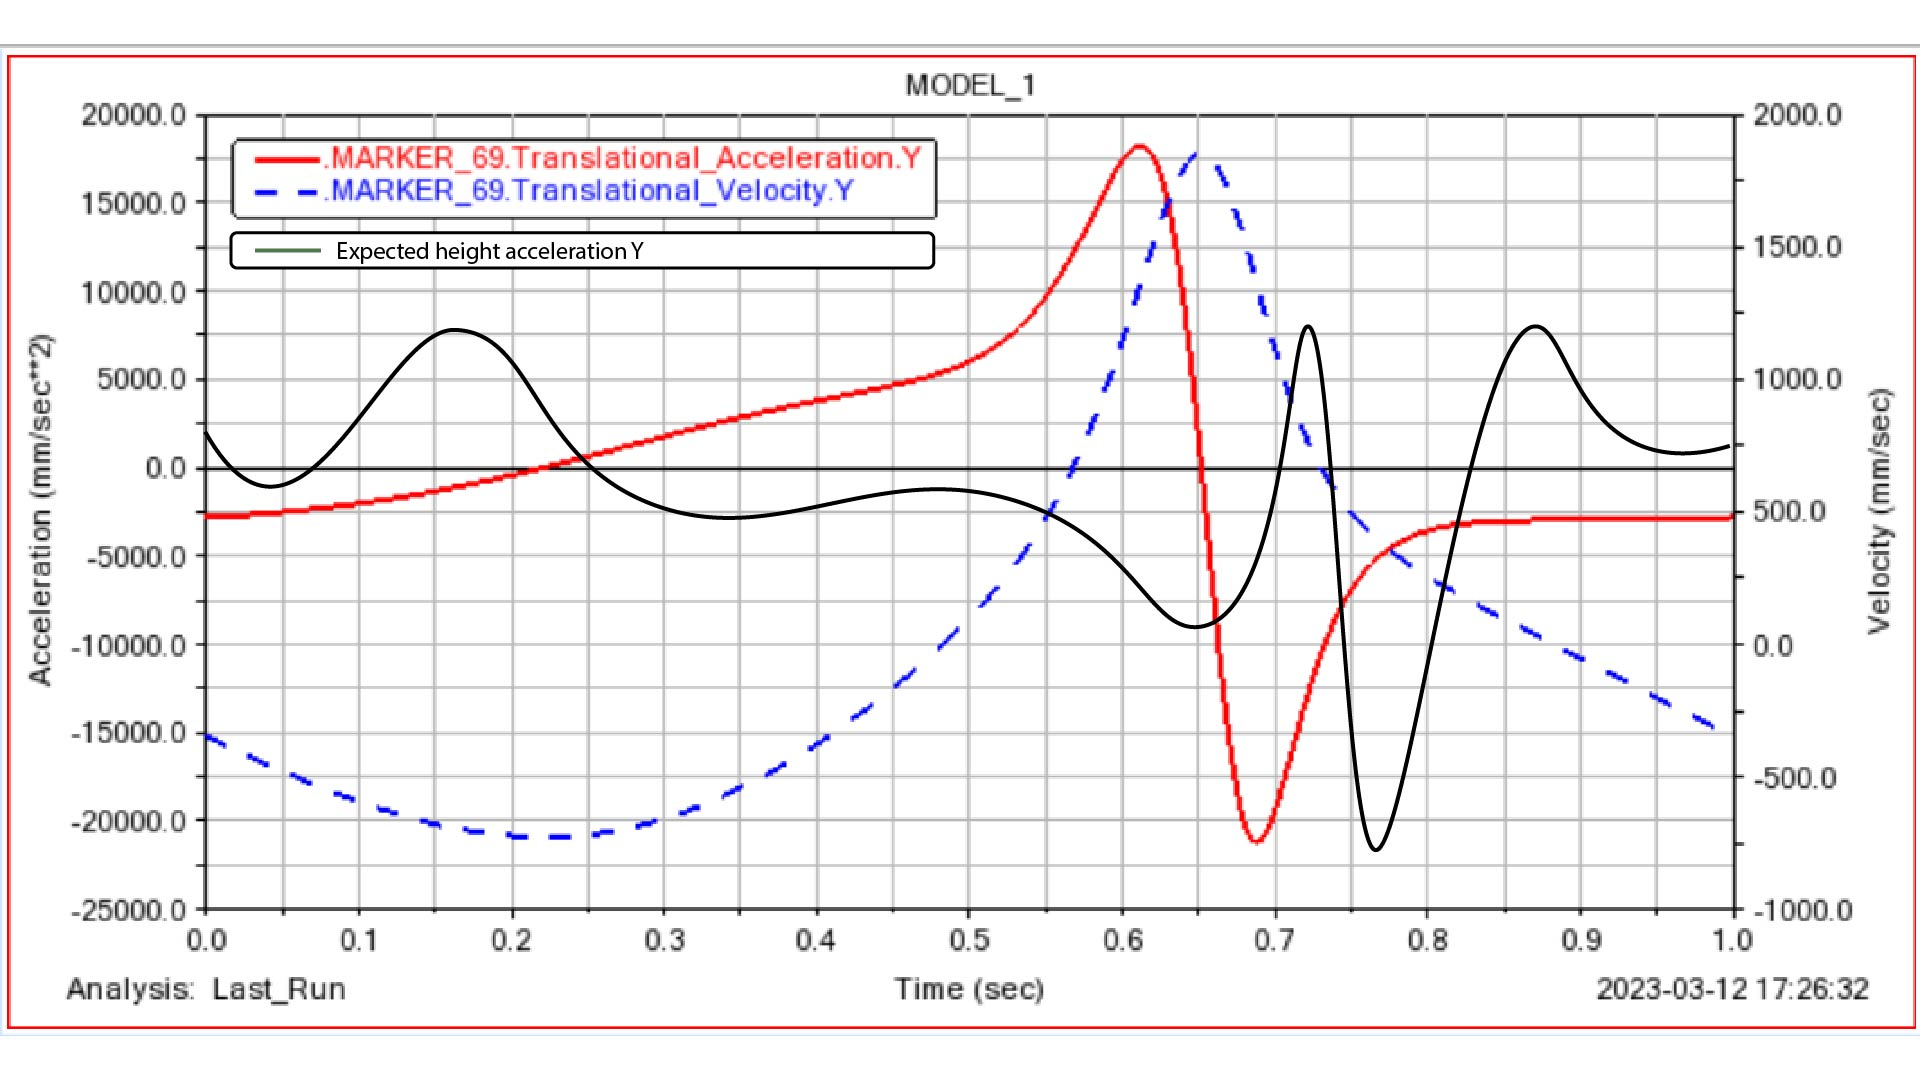
\includegraphics[width=0.9\columnwidth]{Images/height_acceleration madhav-01.jpg}
                \caption{Y Acceleration vs time}
                \label{fig:y_acc}
            \end{figure}

        \subsubsection{Comments}
            Explaining the dissimilarity between simulated and expected plots if any.
            \begin{enumerate}
                \item The slight dissimilarity between the simulated and expected displacement is due to various reasons.
                \item The chain drives have been approximated to be large gears.
                \item Expected graph assumes non circular gears made for desired output trajectory, but in most of the mechanisms and my mechanism used a 4-bar mechanism at the end to generate similar trajectory with part of the coupler as the output.
                \item The error in velocity profiles builds up from the displacement profile by differentiation. Due to discrete time differentiation we know that the error due to noise increases rapidly. So it is possible that the expected values have noise.
                \item Similar explanation goes for acceleration error.
                \item The error also comes from different dimensions assumed during modelling of the mechanism as certain dimensions from the original mechanism were unknown. 
            \end{enumerate}

    \subsection{Sensitivity Analysis}
        Study of the sensitivity of the kinematic parameters of the output component to small changes in the dimensions (e.g. link lengths) of the two other components. The additional graphs with the modified components which were used for performing this sensitivity analysis is shown along with the original graphs.

    \subsection{Analysis of joint clearance}
        Introducing a clearance in one of the joints and simulating the mechanism to run at normal speed and at higher speed. 

        \subsubsection{Normal speed}

        \subsubsection{Higher speed}